The hyperparameters of the models were optimized using Bayesian optimization.
Due to the very large dataset and the time constraint, all models were run for 100 iterations with an early stopping rounds of 10 during the optimization phase. 
However, during the training phase, all models were run for 1000 iterations with an early stopping rounds of 20, in order to maximize the learning done by the models.
On another note, for the LSTM and MLP models, optimizing the number of layers and the number of nodes per layer at the same time using Bayesian optimization is not a straightforward task.
In order to optimize these hyperparameters, Bayesian optimization was given a specific model structure, in which the number of nodes decrease by a certain factor when going from the last hidden layer to the first.
The Bayesian optimization was then used to optimize the number of layers, the number of nodes for the last hidden layer, as well as the decay rate of the number of nodes.
As a result, Baysian optimization did not have full flexibility over the model's structure. 
For example, a model with three layers and 64, 128, 128 nodes per layer cannot be created using the model structure described, and hence, it is possible that another model exists with a better performance that does not follow the specified model structure.
Moreover, different model structures have different learning patterns depending on their complexity. 
Simple models are able to learn quickly but plateau at a higher error value, whereas complex models learn slowly but can plateau at a lower error value.
Since the models were only ran for 100 iterations and 10 early stopping rounds during the optimization phase, it is possible that a better but more complex model did not have enough time to plateau.
Therefore, a better model can possibly be found by giving more flexibility over the structure of the model, exploring a higher range of values for each hyperparameter, as well as increasing the number of iterations and early stopping rounds during the optimization phase.

Furthermore, looking at Figures \ref{fig:lstm_worst}, \ref{fig:ann_worst}, \ref{fig:lgbm_worst}, and \ref{fig:hyb_worst}, we can see that the models have a difficult time forecasting the sales for the \texttt{FOODS\_3} department.
This shows that items in the \texttt{FOODS\_3} department do not follow the same patterns as the other items.
This can be confirmed by examining Figure \ref{fig:dept_sales}, which shows the difference in the patterns of sales between the \texttt{FOODS\_3} department and the other departments.
Not only do the items in the \texttt{FOODS\_3} department have higher sales, but they also show a seasonality pattern that is less visible in the other departments.
Hence, a possible way to improve forecasting accuracies is to train a separate model for items belonging to the \texttt{FOODS\_3} department.

LSTM models have a high reputation in learning from time-series data. 
However, the LSTM model did not perform as well as expected in this project.
This can be due to the fact that recurrent neural networks, such as LSTM, require extensive non-sparse data.
However, in our case, the data contains many zeros, which can significantly hinder the performance of the LSTM model.
Moreover, the LSTM model was very sensitive to the values of its hyperparameters, and hence, it requires extensive hyperparameter optimization.
On the other hand, LightGBM models are easy to train and are able to achieve a relatively good performance without much hyperparameter optimization.
Although the results of the LGBM model are noteworthy and show the strength of boosting methods in improving the overall performance, it is possible that a well optimized LSTM model can outperform the LGBM model, however, this would require a considerable amount of hyperparameter optimization.

Similarly, the hybrid model was not able to meet expectations. 
The performance of the hybrid model seemed to be very closely tied to the performance of its first component, LSTM, which is possibly due to the fact that the first component receives the main sales data and hence carries out the main learning in the model.
Moreover, although the second component, LGBM, was able to slightly improve the accuracy of the 28-days ahead forecasts, it was not able to learn much from the residual data that was provided and seemed to have a difficult time finding a pattern and predicting the error of the LSTM model.
Therefore, it could be possible for the hybrid model to beat the performance of its two individual components, however, its first component will need to perform at least as good as its second component when used as a singular model, since the first component will be doing the main learning in the hybrid model.
Furthermore, another possible way to improve the performance of the hybrid model is to perform hyperparameter optimization on its two components.
In this project, the hyperparameters of the singular models were used in the hybrid model.
Since the input data for the two components are similar to the input data of the singular models, this can be considered a case of transfer learning, and hence the same hyperparameters should be able to perform relatively well.
However, with further hyperparameter optimization, we should still be able to find better hyperparameters for each component of the hybrid model.
Nevertheless, hybrid models are not guaranteed to outperform singular models and model selection has a significant influence on their performance as well \cite{c12}.

Another factor to consider when evaluating the performances is the choice of features used.
The main data for the LSTM model included the sales time-series for each item, which is what the model will be predicting. 
In order to help with the predictions for the singular LSTM model, seven other features were used from the dataset, and two additional features were introduced. 
The seven features used from the dataset include the current day number, weekday, month, year, SNAP days for California, SNAP days for Texas, and SNAP days for Wisconsin. 
Moreover, two additional features were created from the available events data, which represented whether an event exists on the day of the prediction, and whether an event exists the day after the prediction.
The reason that the model was provided with information about the events of the next day is that people tend to go shopping before an event rather than the day of the event.
For example, in case of Halloween, a lot of people tend to buy their candies before Halloween starts rather than on the day of Halloween.
Moreover, we also tried providing the model with the price information of each item, as well as the exact name and type of each event, however, the performance of the LSTM model was significantly hindered, and hence, these features were omitted.
This is possible due to the large number of features added, since there is a new feature added for the price of each item, and hence, we are essentially doubling our feature set.

\begin{figure}[b!]
    \centering
    \fbox{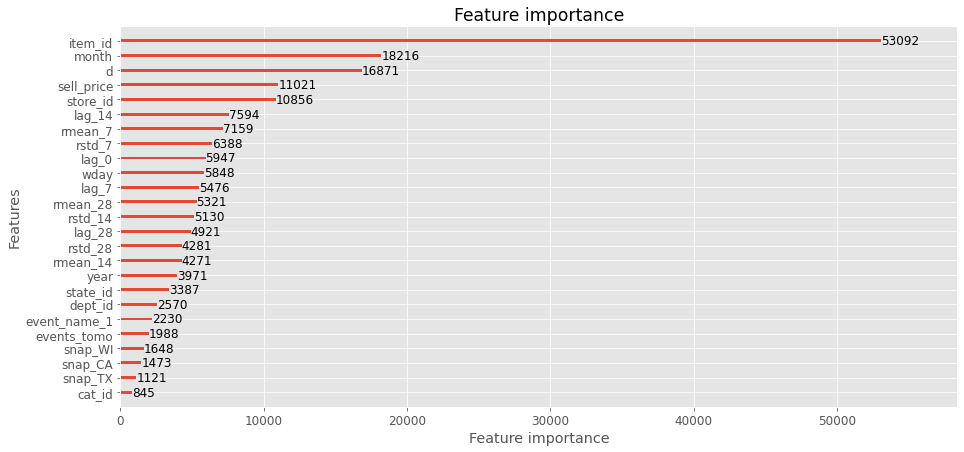
\includegraphics[width=0.95\textwidth]{figures/results/feat_importance.png}}
    \caption{The importance of each feature obtained from the LGBM model.}
    \label{fig:feat_imp}
\end{figure}
For the MLP and LGBM models, all available features were used. In addition, the lag of sale values with intervals 28, 35, 42, and 56 days, and the rolling mean and standard deviation of the sale values with window sizes 7, 14, and 28 days and a lag of 28 days were introduced.
Figure \ref{fig:feat_imp}, which was obtained from the singular LGBM model, shows a list of these features and their significance in attaining the predictions.
Note that all lag and rolling mean/std features were shifted by 28 days, since we have a forecasting horizon of 28 days.
Shifting these features by the value of the forecasting horizon prevents the error of the model to propagate through later predictions.
For example, if we introduce a lag feature with an interval of 7 and try to predict 28 days ahead, we will not have the actual sale values after the seventh forecast and we will have to use the predicted values instead. 
This means that if there is an error in the predictions, the error will propagate through later forecasts as well.
However, we also tried providing the MLP and LGBM models with lag and rolling mean/std features that are within the forecasting horizon. 
Even though this boosted the performances on the 1-day ahead forecasts, it significantly hindered the performances on the 28-days ahead forecasts.
Although, it is important to note the importance of recent sales in the foretelling the future sales. 
Having knowledge of recent sale values can greatly help with the predictions, however, this comes with the trade-off of error propagation when forecasting longer horizons.
Therefore, further optimization can be possibly done by providing the models with lag and rolling mean/std features that are within the forecasting horizon and balancing the aforementioned trade-off between the recency of these features and error propagation.
Moreover, the reason that the 1-day and 28-days ahead forecasts of the MLP and LGBM models are the same is the fact that all lag and rolling mean/std features are shifted by the value of the forecasting horizon, and so actual sale values are available for the entire forecasting horizon.
However, this is not the case for the LSTM model, since the LSTM model will have to depend on its own predictions when it has a large forecasting horizon, and hence the LSTM and hybrid models obtain different 1-day and 28-days ahead predictions.